\documentclass[12pt]{article}
\usepackage{graphicx}
\usepackage{placeins}
\title{COP290: User Registration App}
\author{Sai Deep (2012CS10223) \\ Mano Teja (2010CS50286) \\ TRK Saran (2010BB50042) }
\begin{document}
\maketitle
\tableofcontents

\section{Introduction}
Our task was to design an Android application to register teams for COP290 course.
\section{User Interface}
\subsection{Primary Screen}
A scrollable layout with one field for entering team name, 3 fields each for names and entry numbers respectively followed by a \textbf{Register Now} button. 
\begin{figure}[!ht]
	\centering
	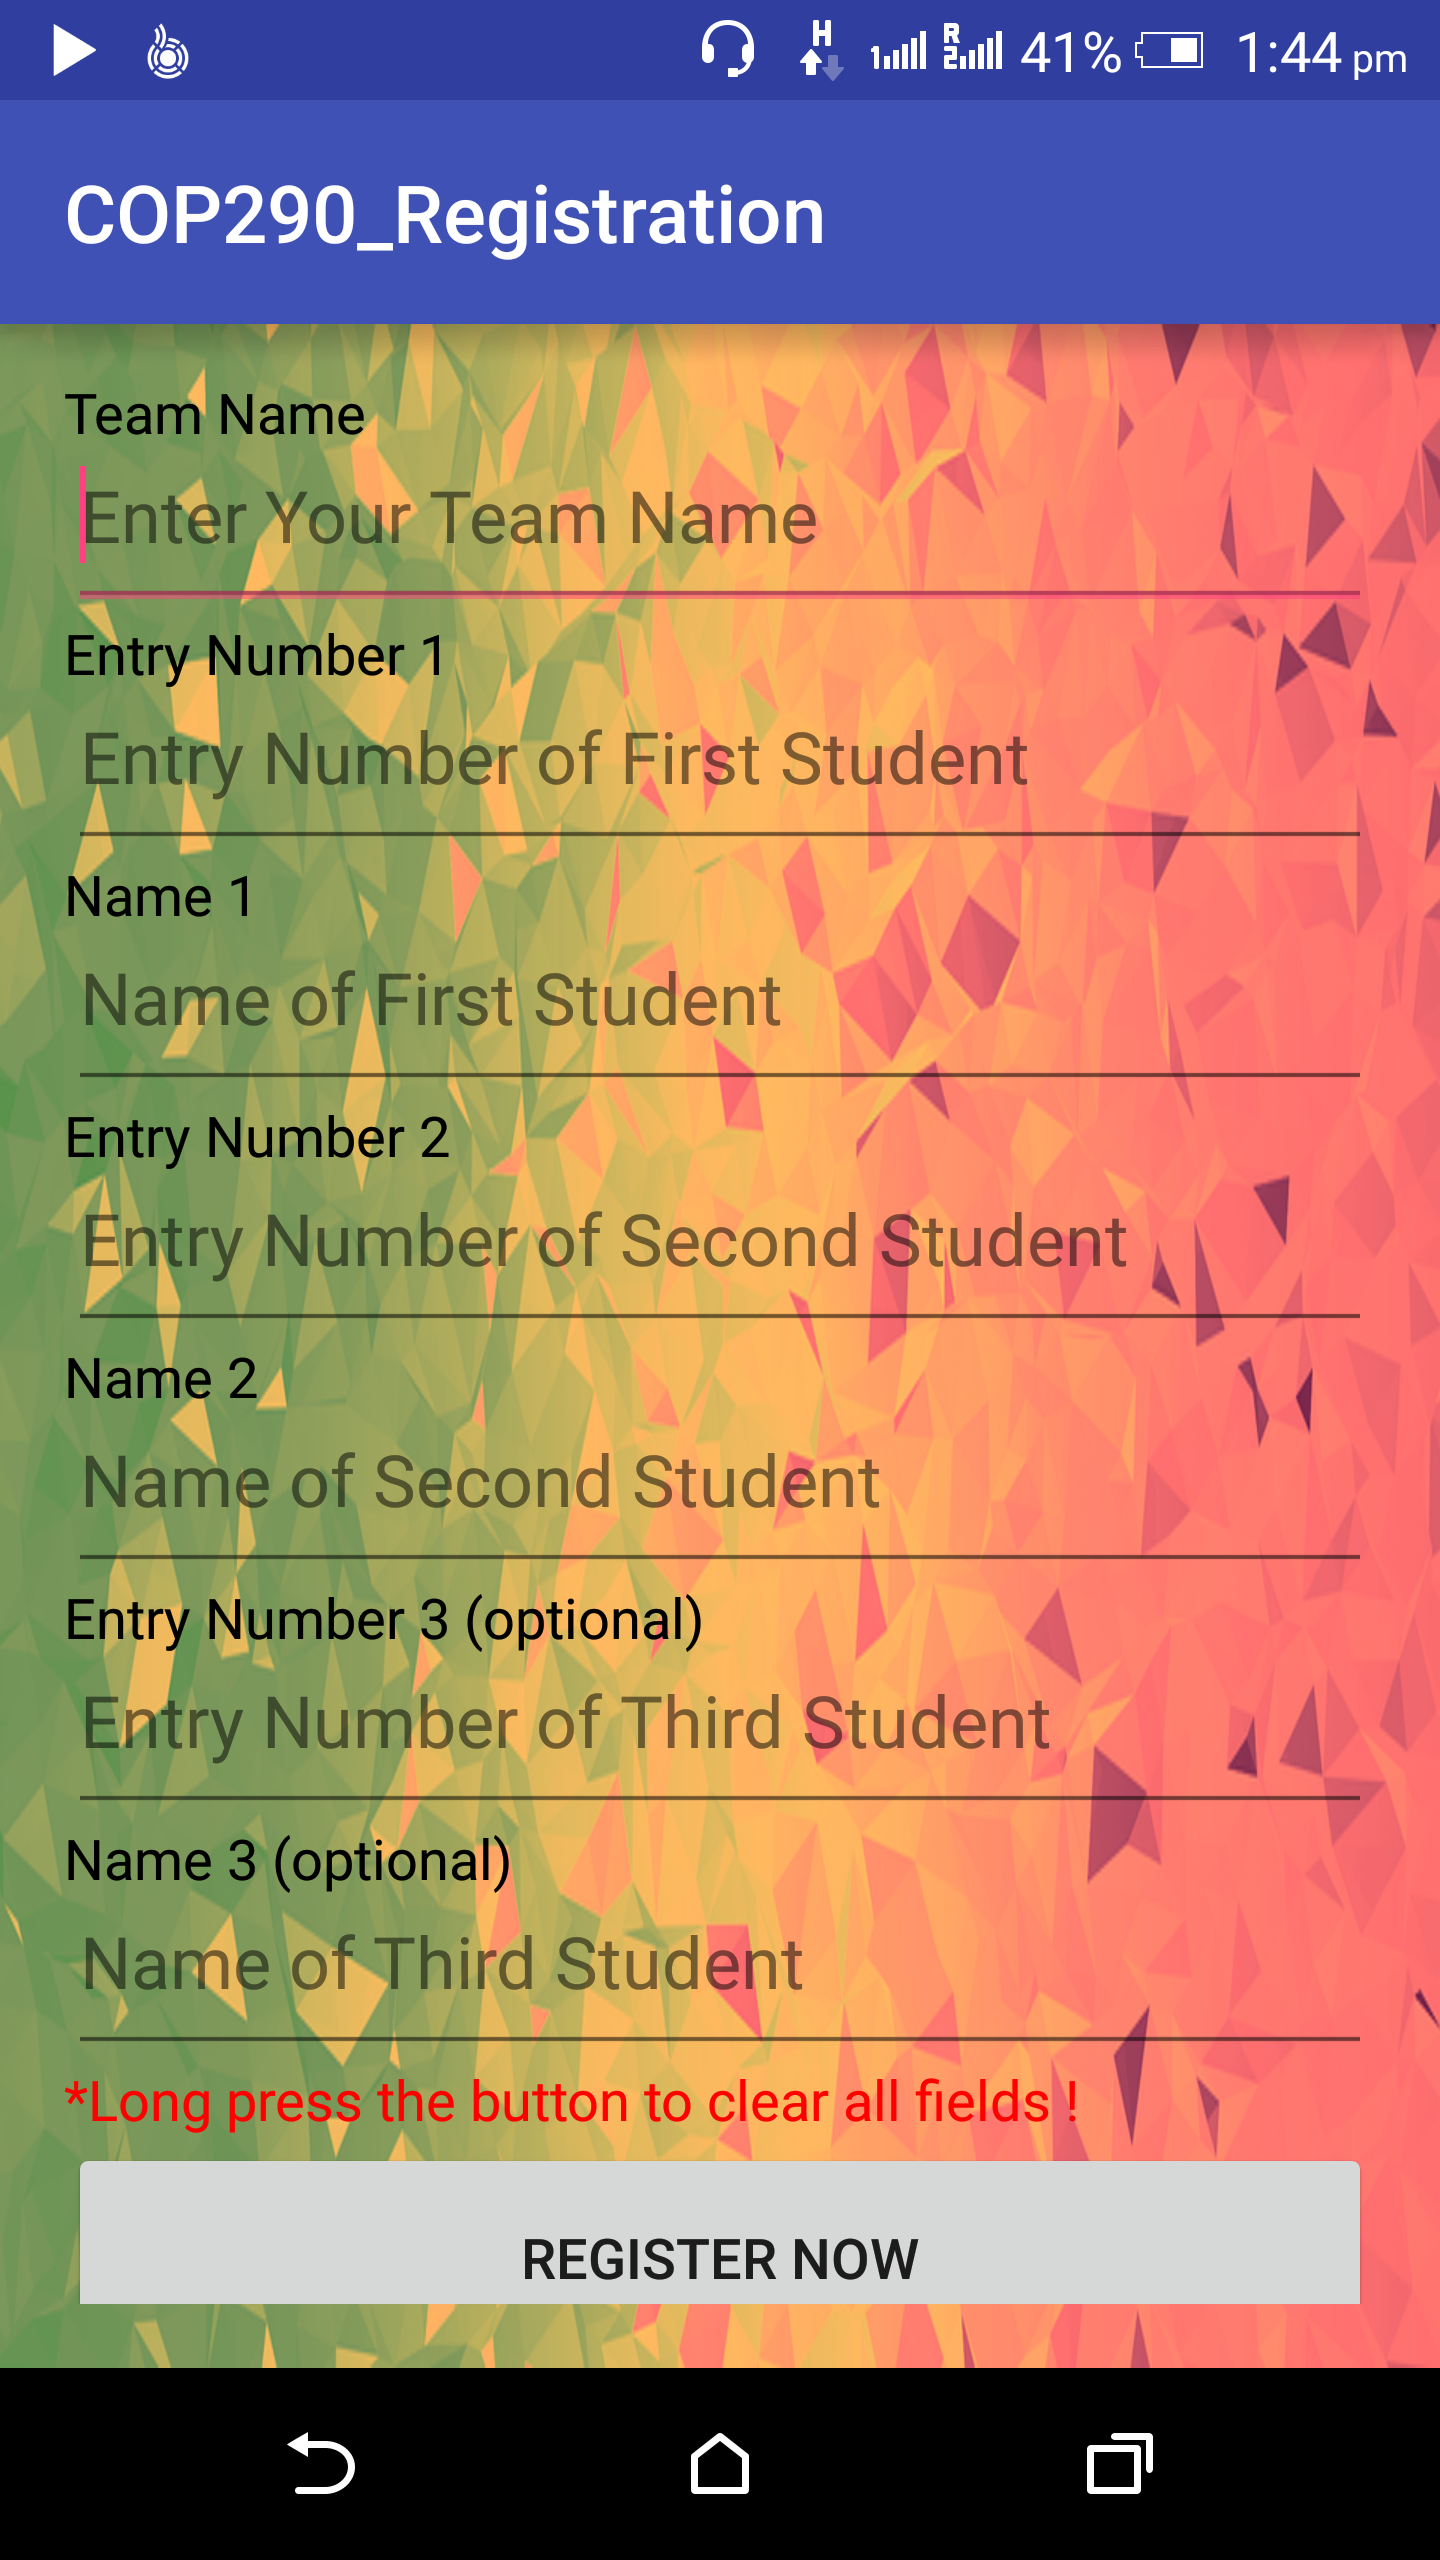
\includegraphics[width=0.5\textwidth]{images/home.png}
	\caption{Primary Screen}
\end{figure}
\subsection{Display of Errors}
The fields are processed one by one. The first invalid text field is highlighted. Subsequent invalid fields are highlighted one by one only after the previous invalid one is corrected.\\   
\begin{figure}[!htb]
  \centering
  \begin{minipage}[b]{0.4\textwidth}
    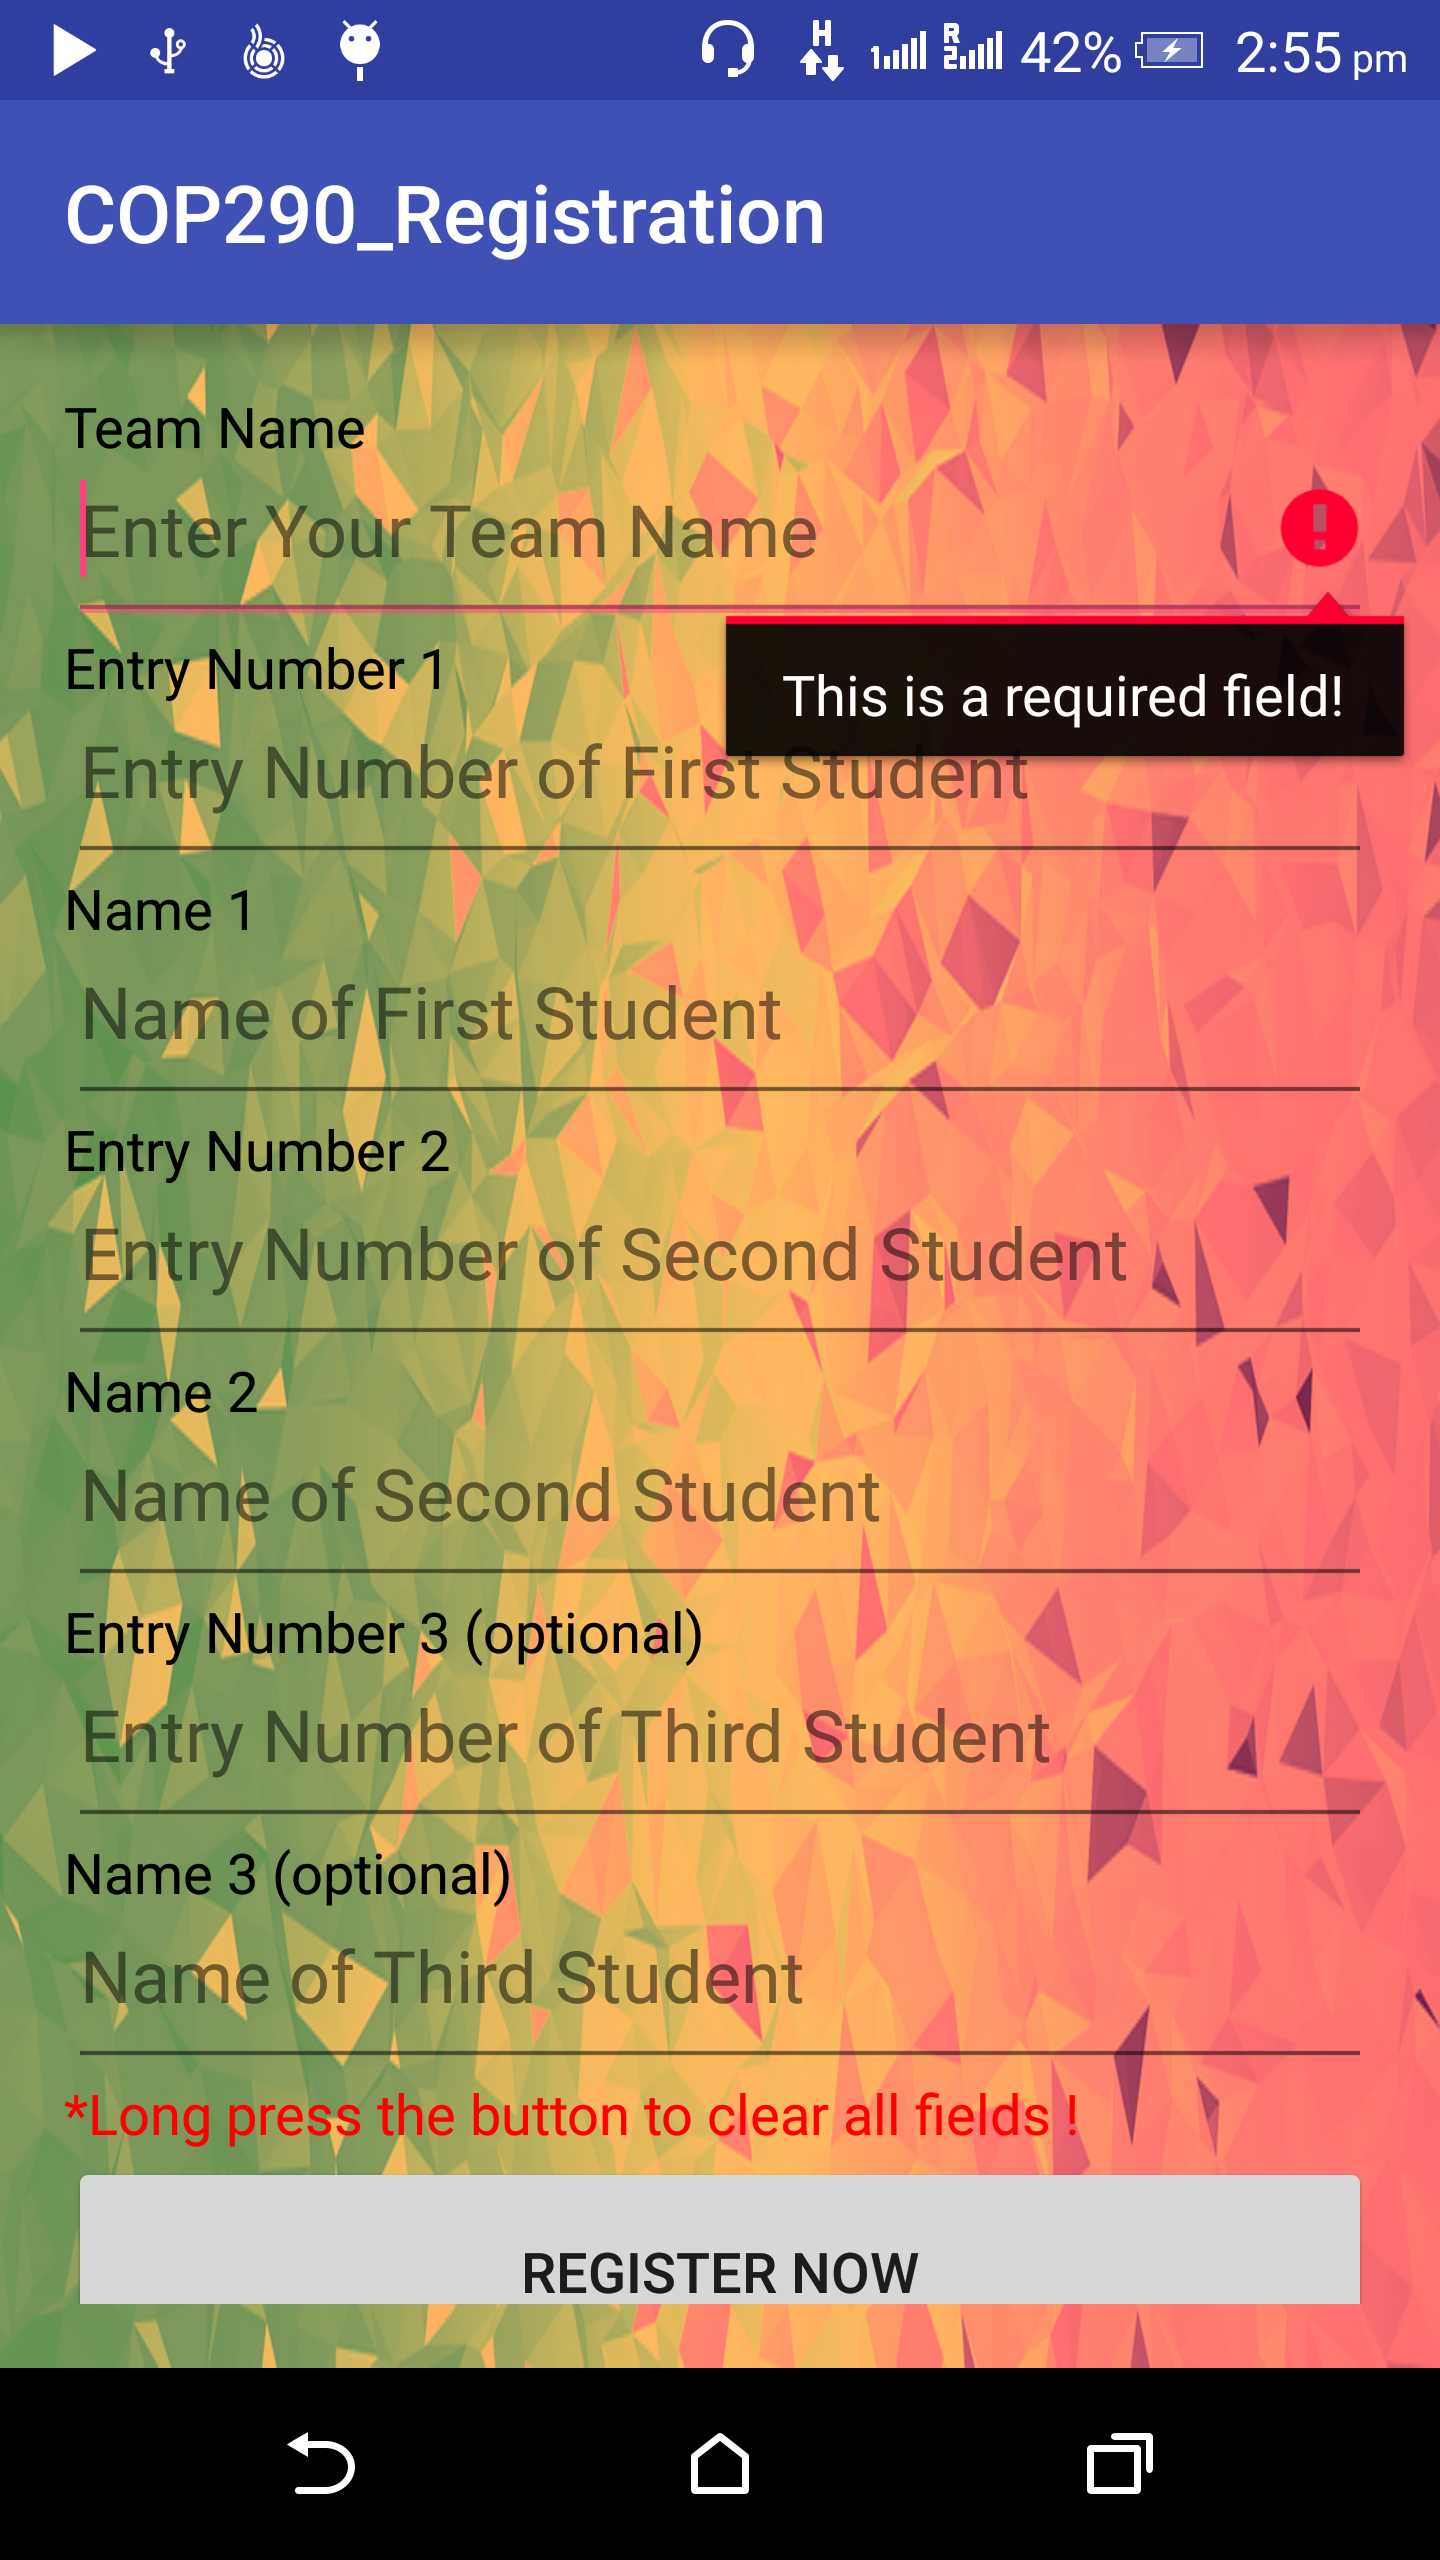
\includegraphics[width=\textwidth]{images/empty.png}
    \caption{Empty field (Applicable for first 5 fields)}
  \end{minipage}
  \hfill
  \begin{minipage}[b]{0.4\textwidth}
    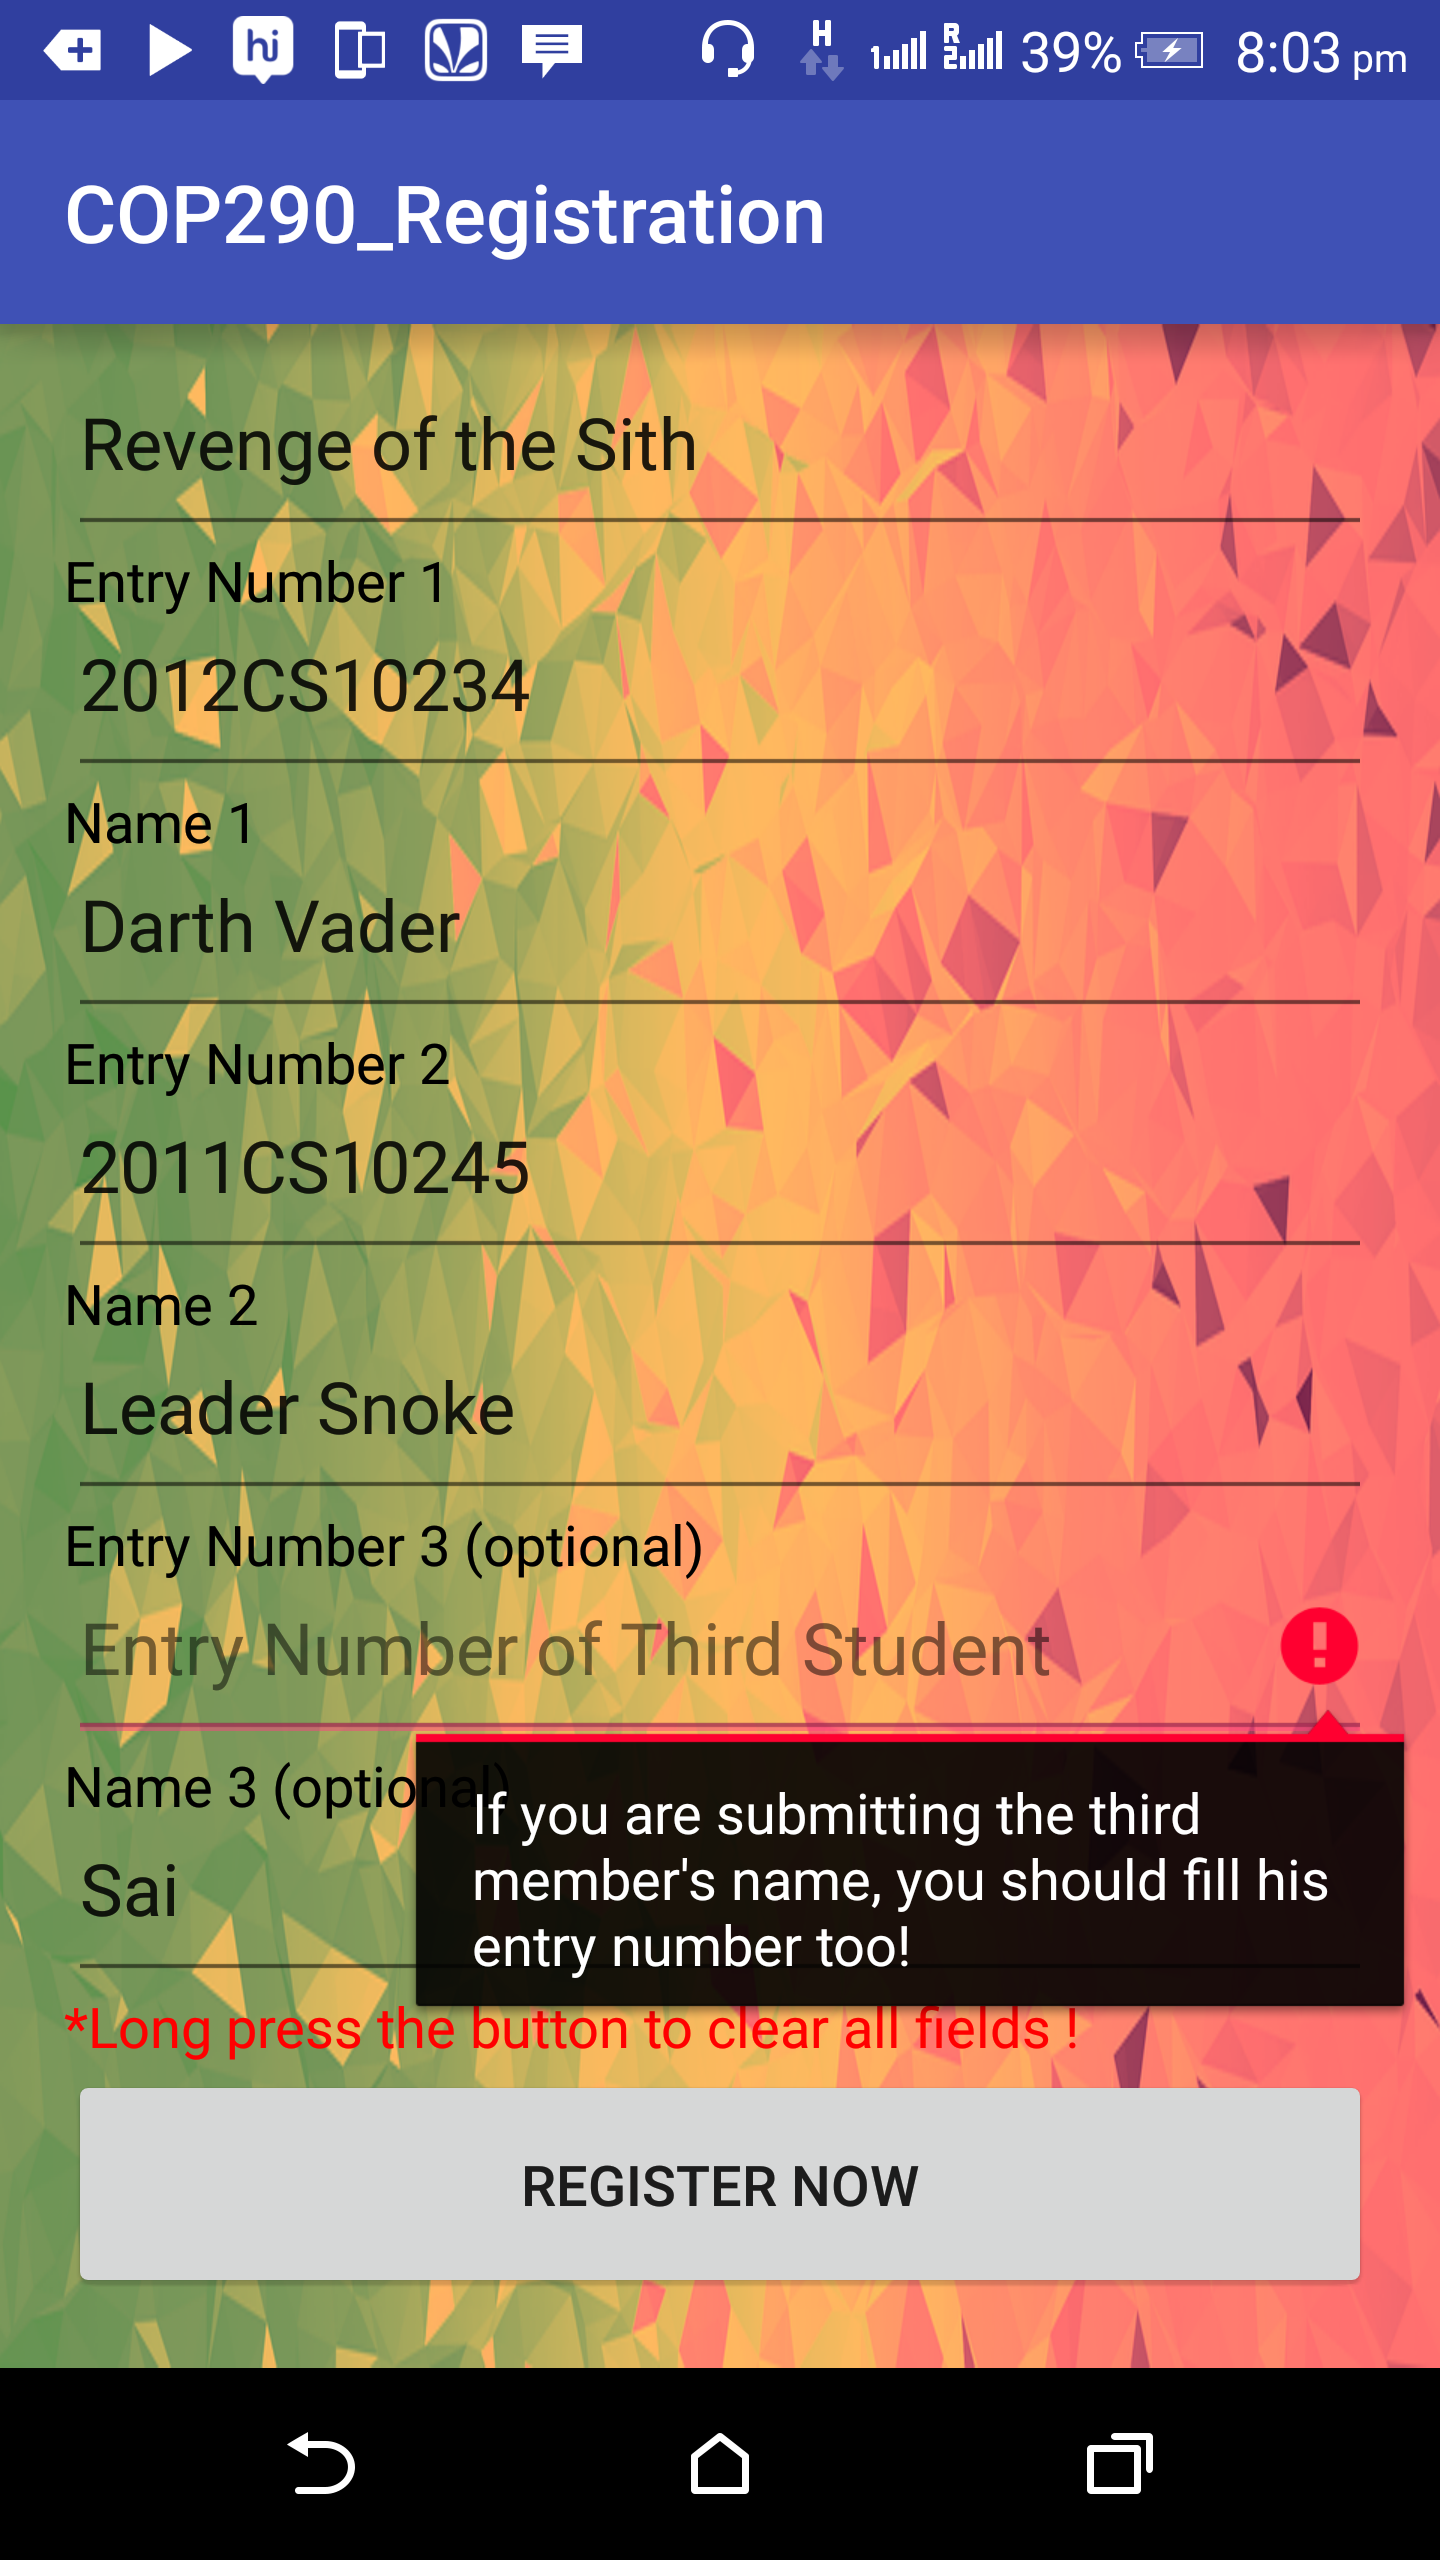
\includegraphics[width=\textwidth]{images/optional.png}
    \caption{When only one of the two optional fields is filled}
  \end{minipage}
\end{figure}

\begin{figure}[!htb]
  \centering
  \begin{minipage}[b]{0.4\textwidth}
    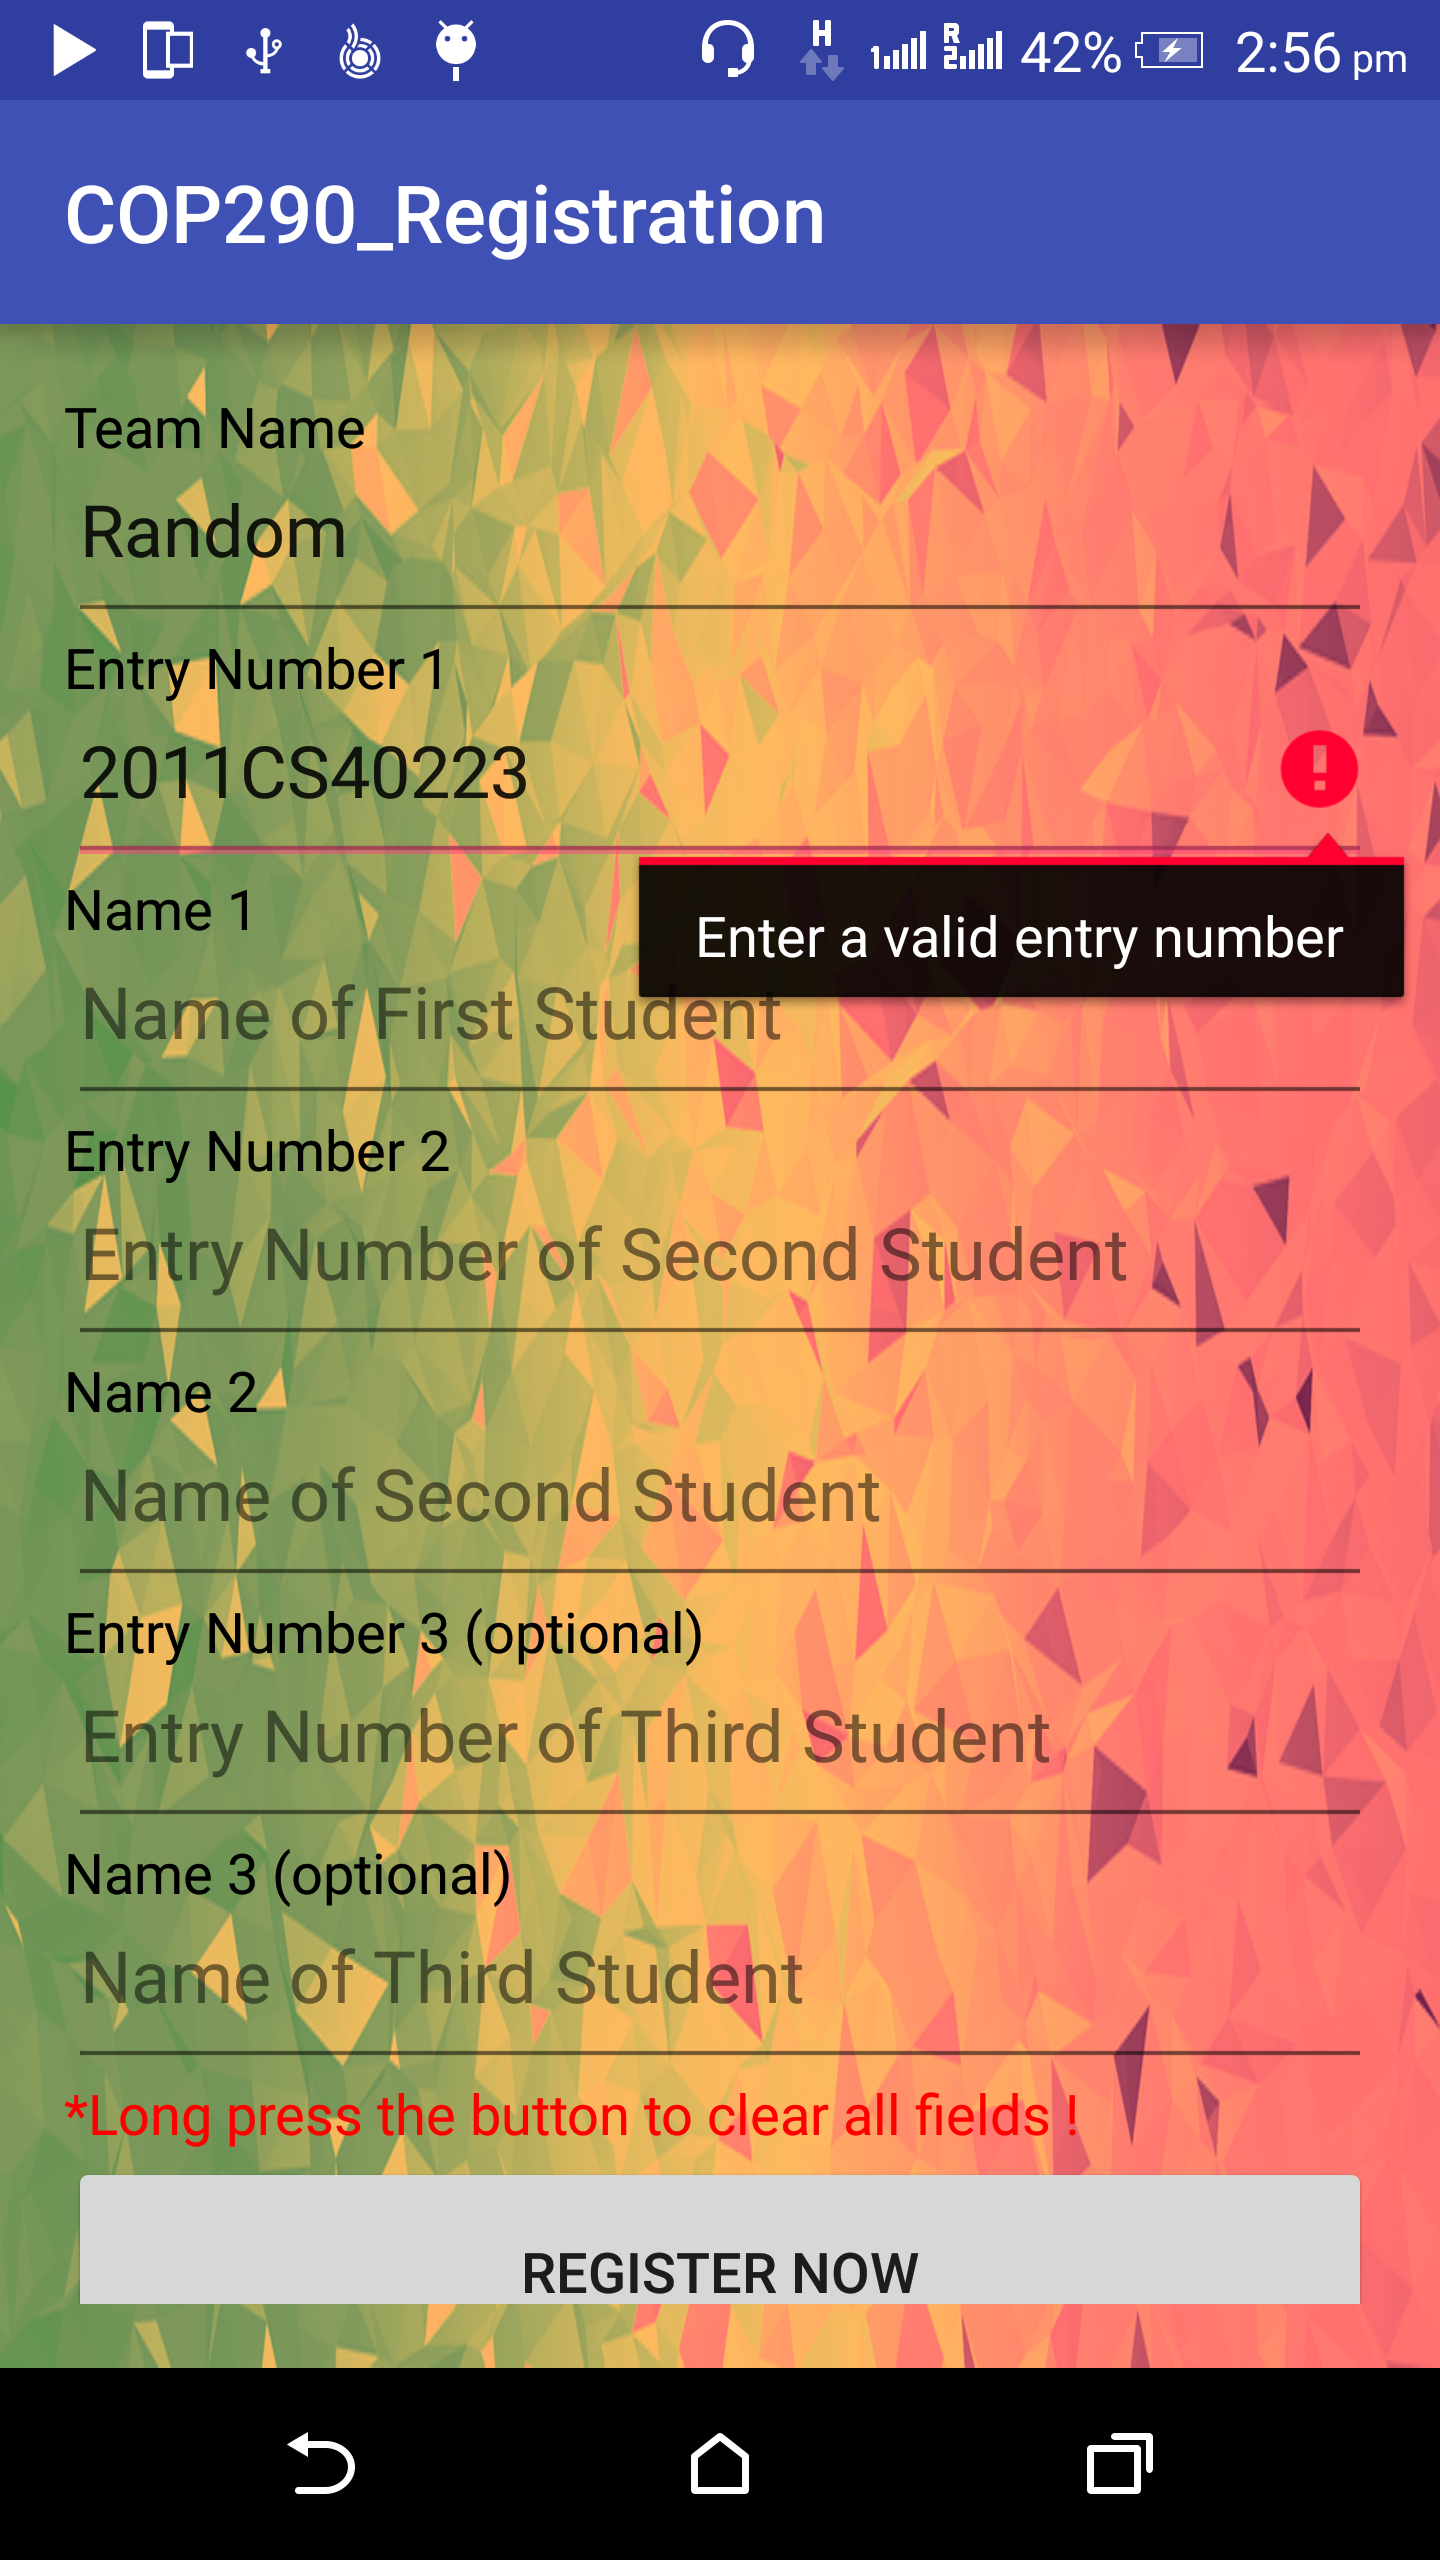
\includegraphics[width=\textwidth]{images/invalidentry.png}
    \caption{Invalid Entry}
  \end{minipage}
  \hfill
  \begin{minipage}[b]{0.4\textwidth}
    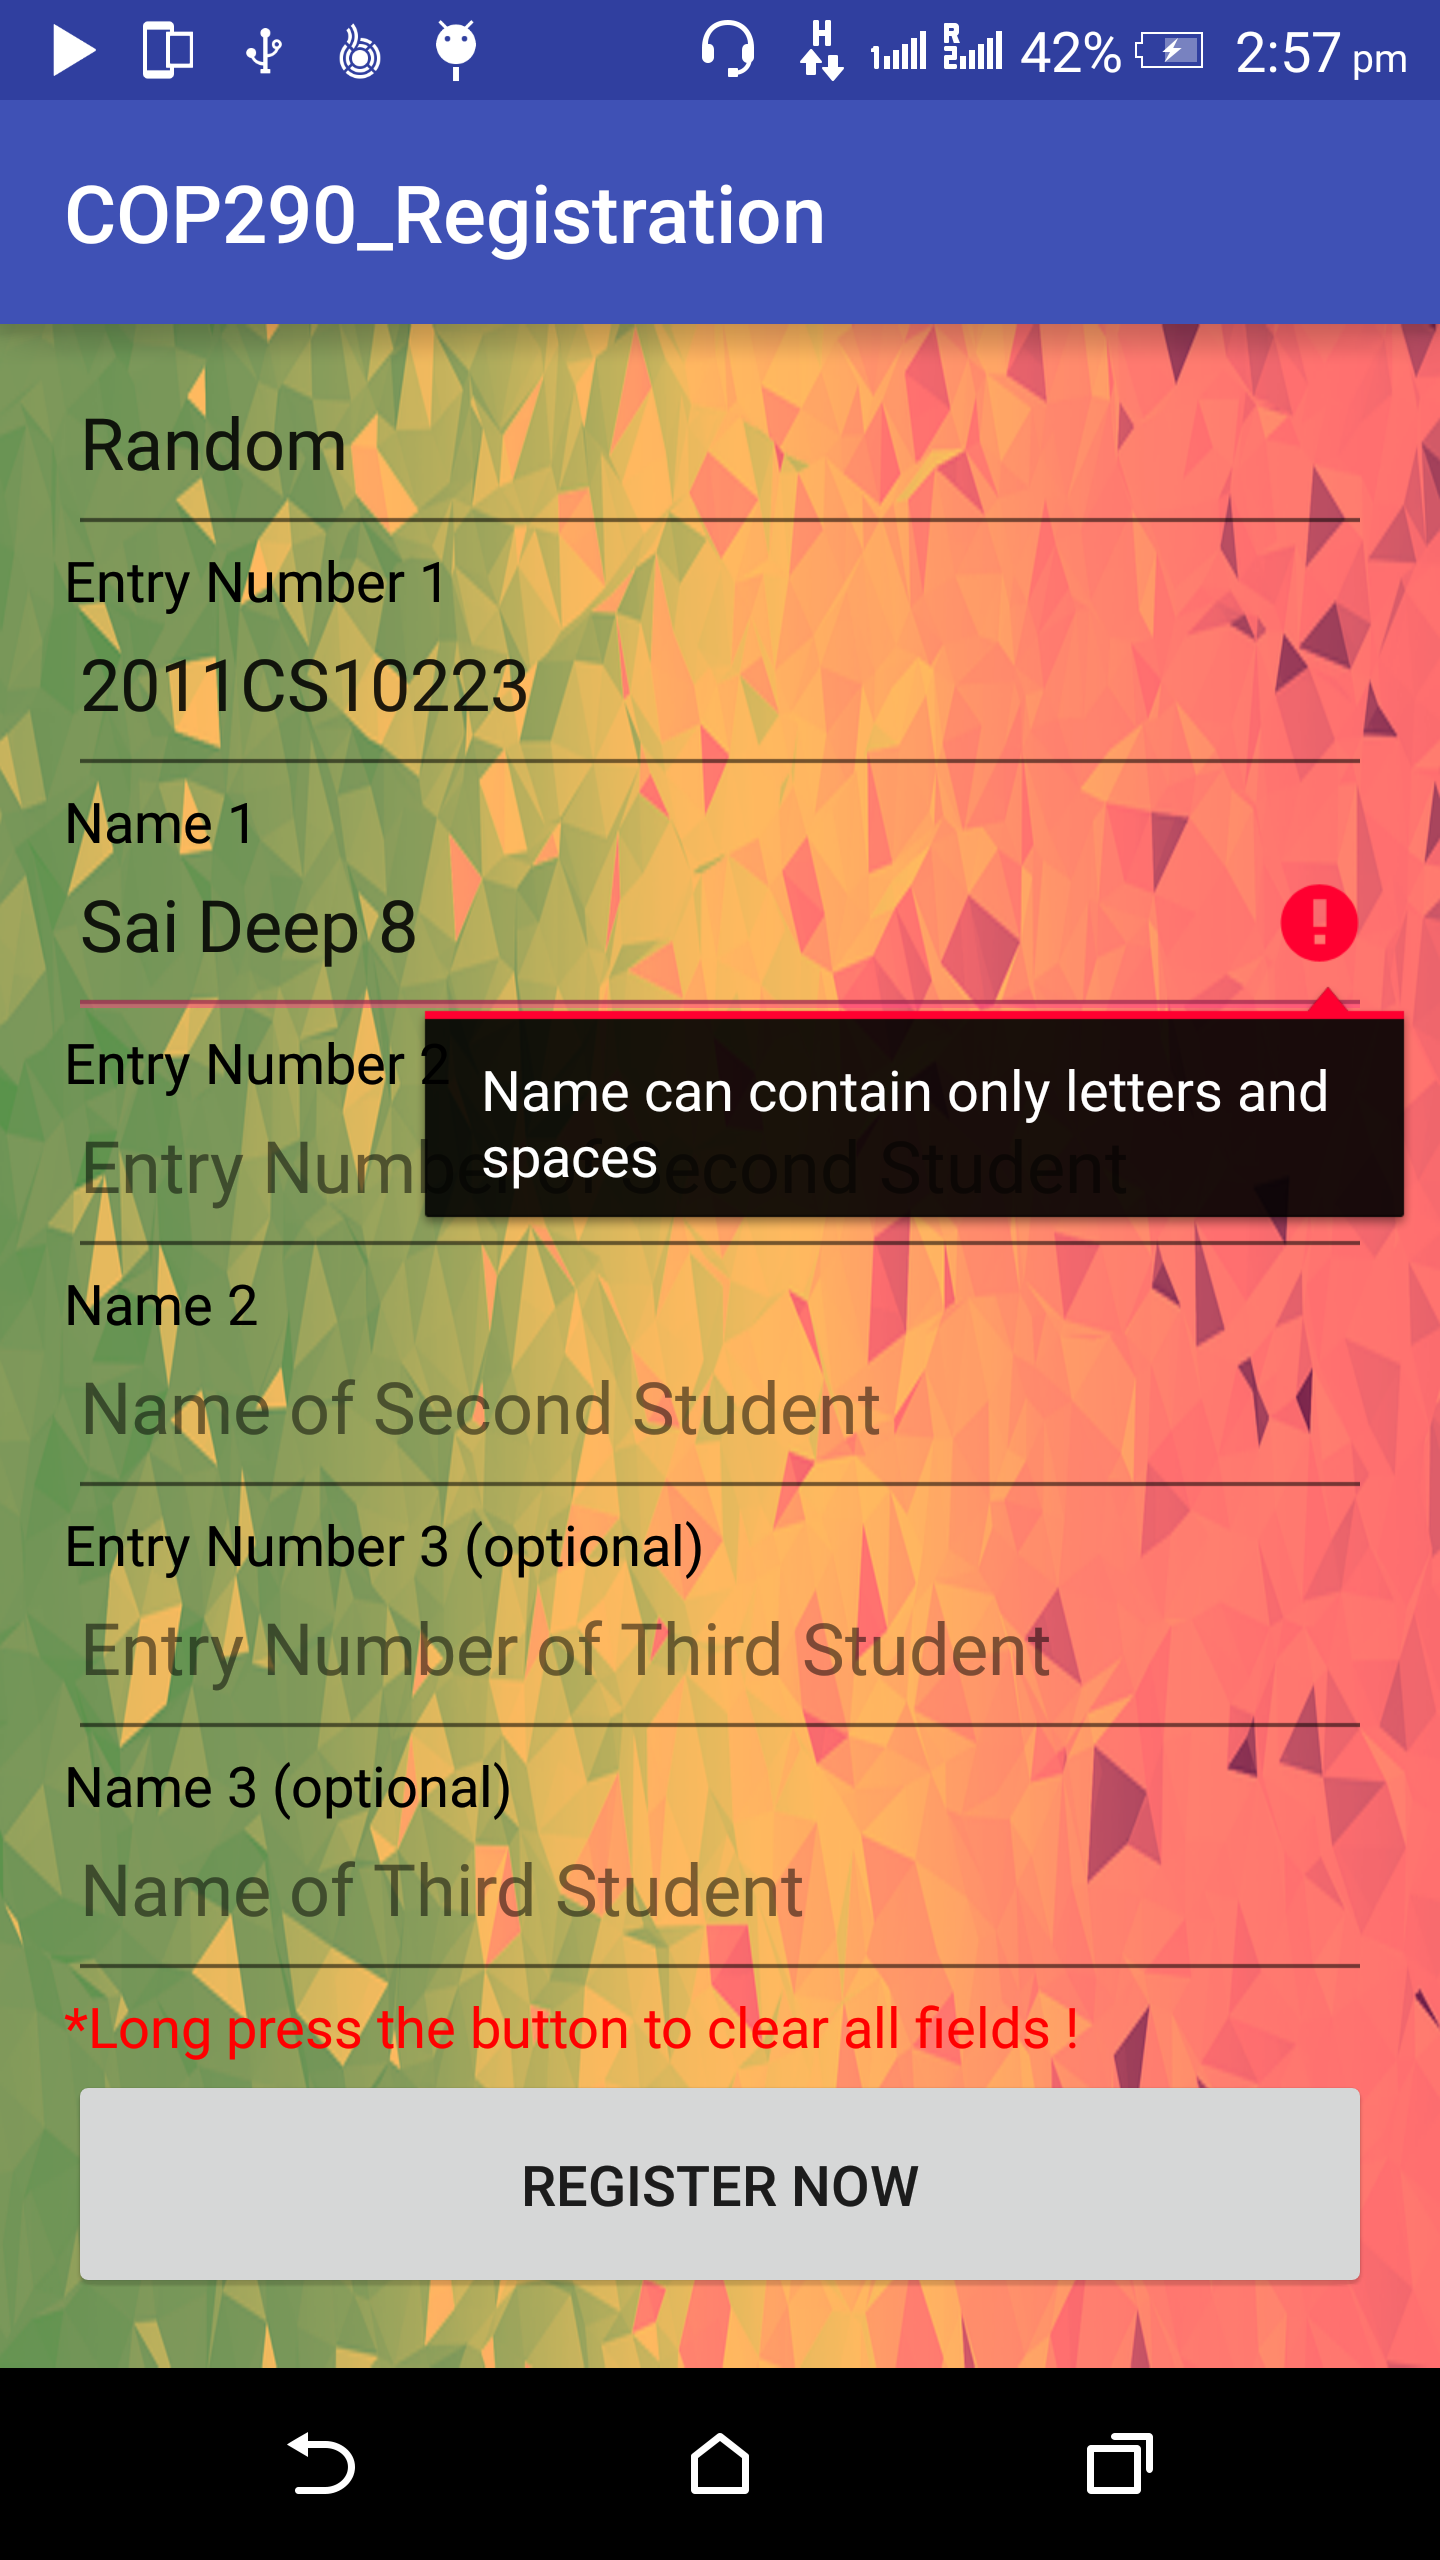
\includegraphics[width=\textwidth]{images/invalidname.png}
    \caption{Invalid Name}
  \end{minipage}
\end{figure}

\FloatBarrier
\subsection{On Pressing Register Button}
Register button sends the data to server only if all the entered fields are valid. Below are the screens illustrating possible responses from the server which is shown as a toast message.

\begin{figure}[!htb]
  \centering
  \begin{minipage}[b]{0.4\textwidth}
    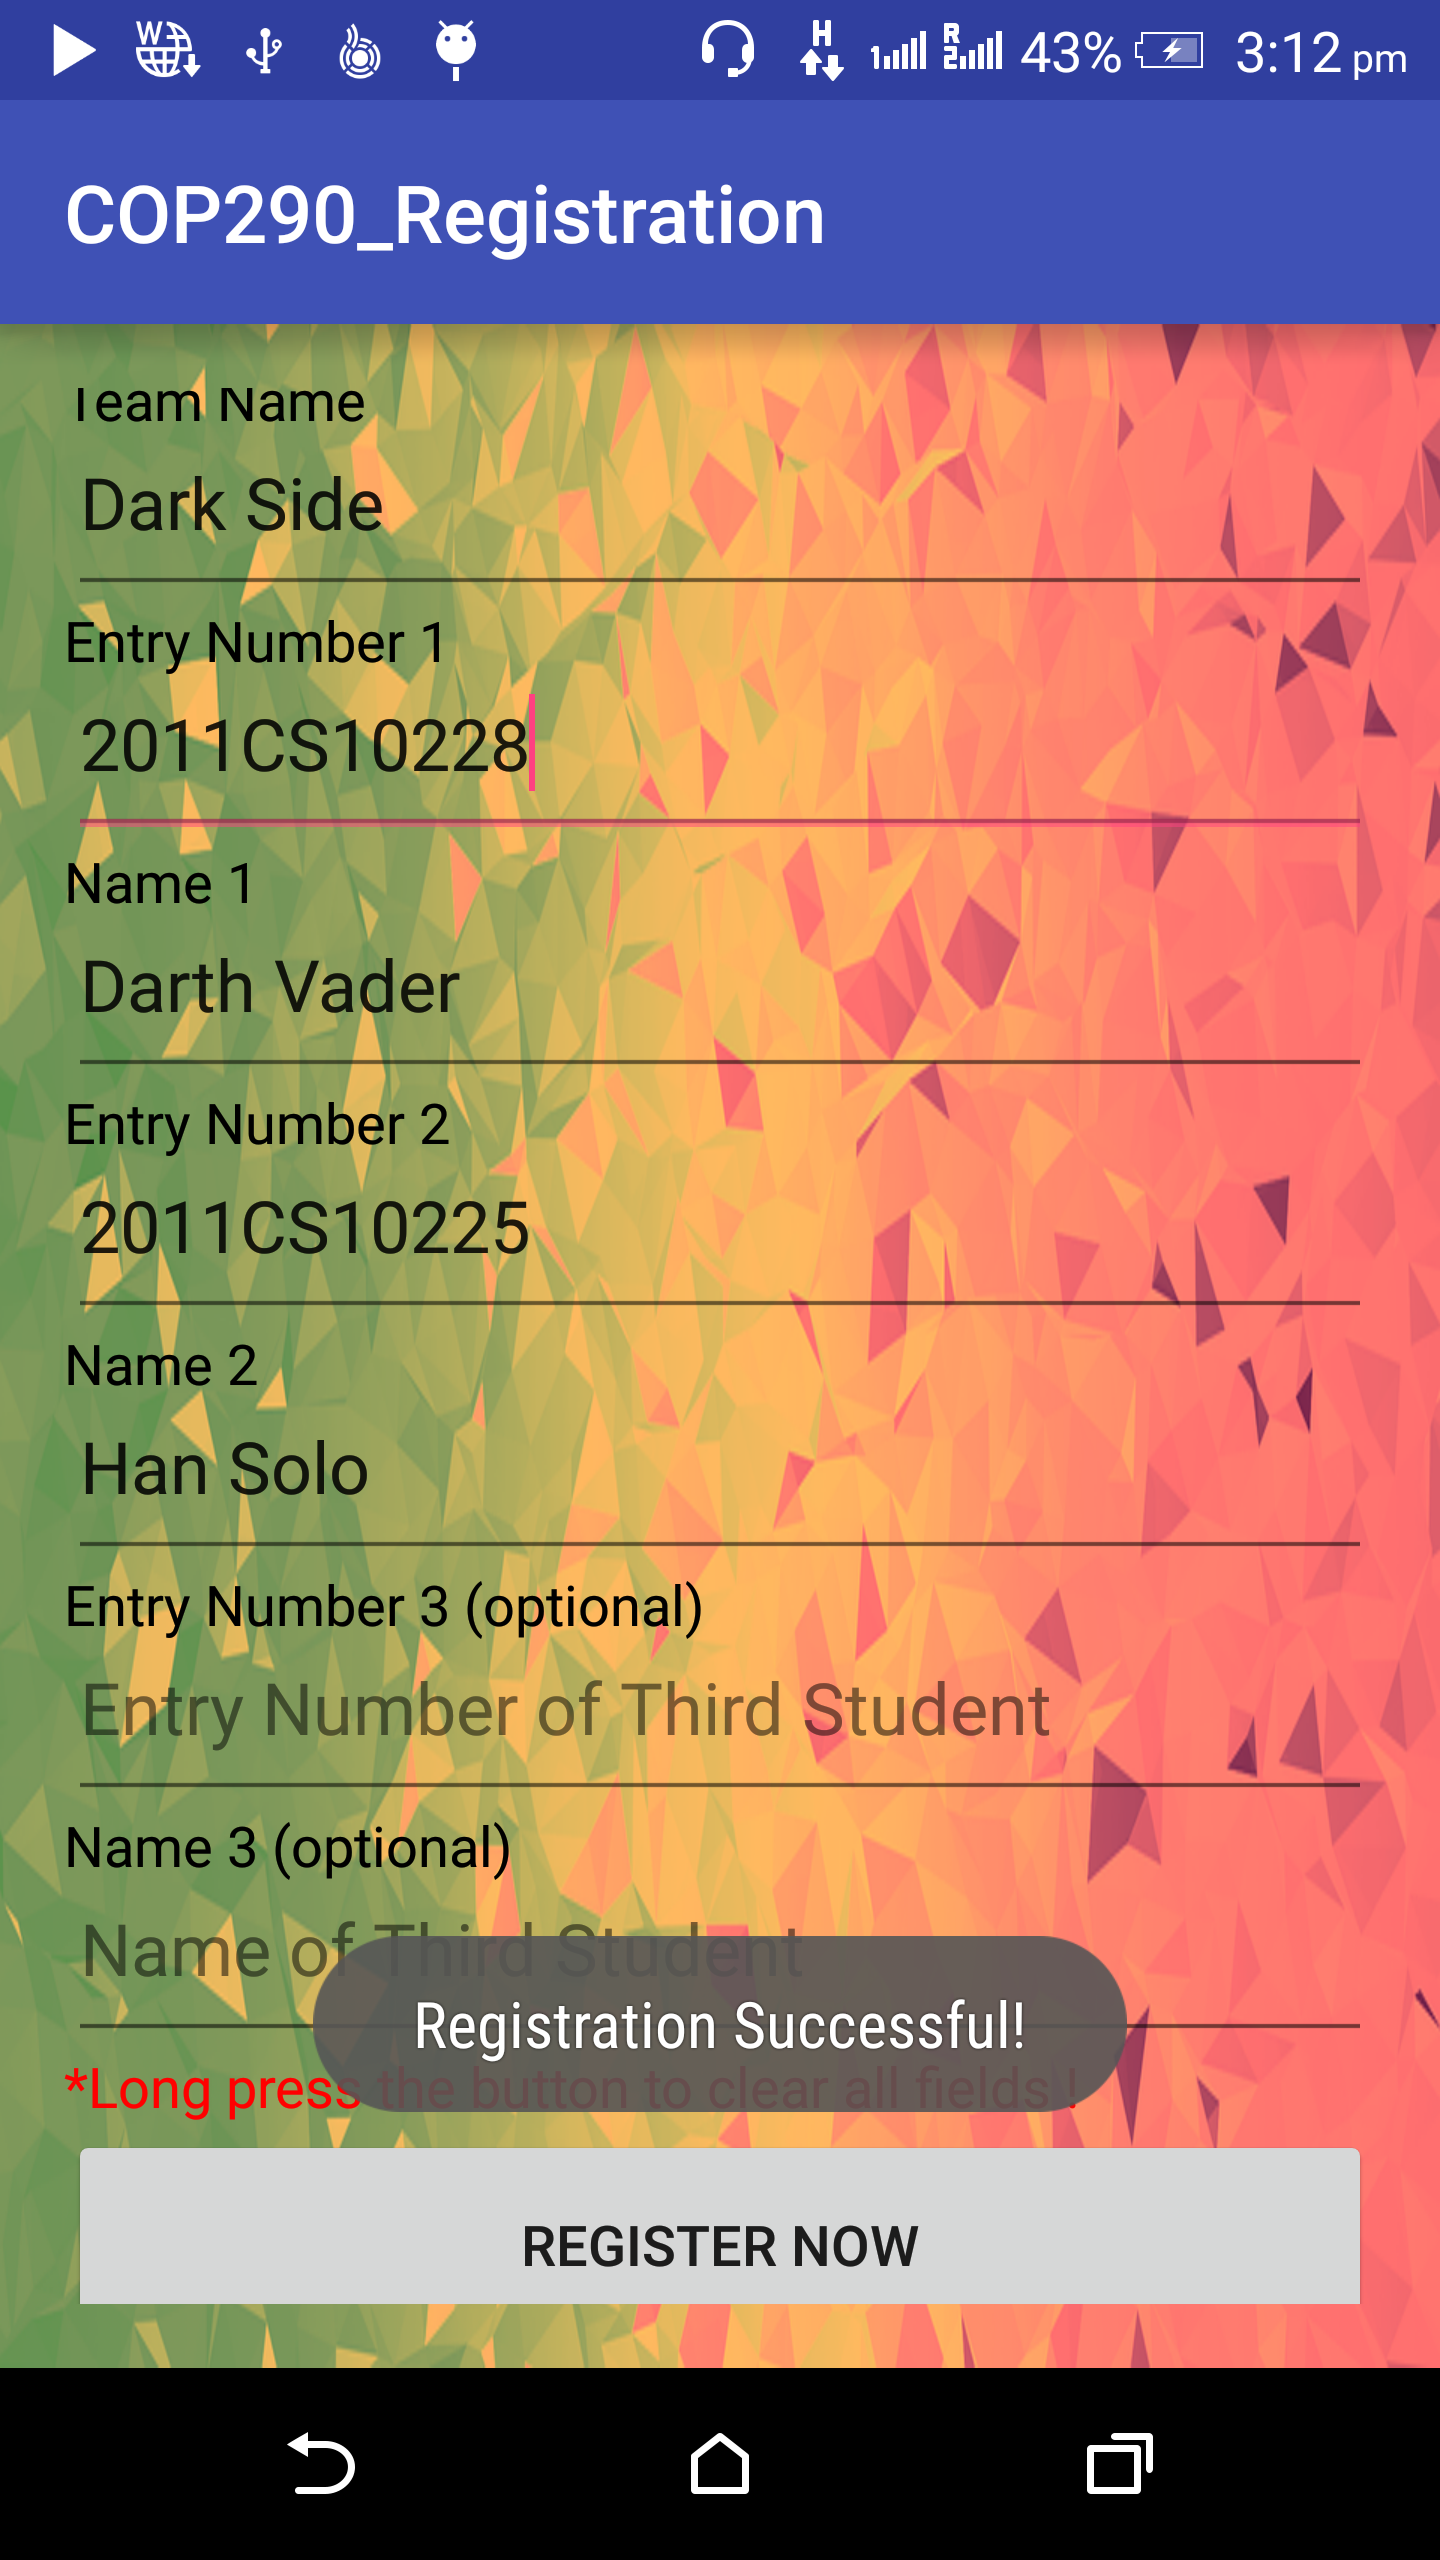
\includegraphics[width=\textwidth]{images/success.png}
    \caption{Successful Registration}
  \end{minipage}
  \hfill
  \begin{minipage}[b]{0.4\textwidth}
    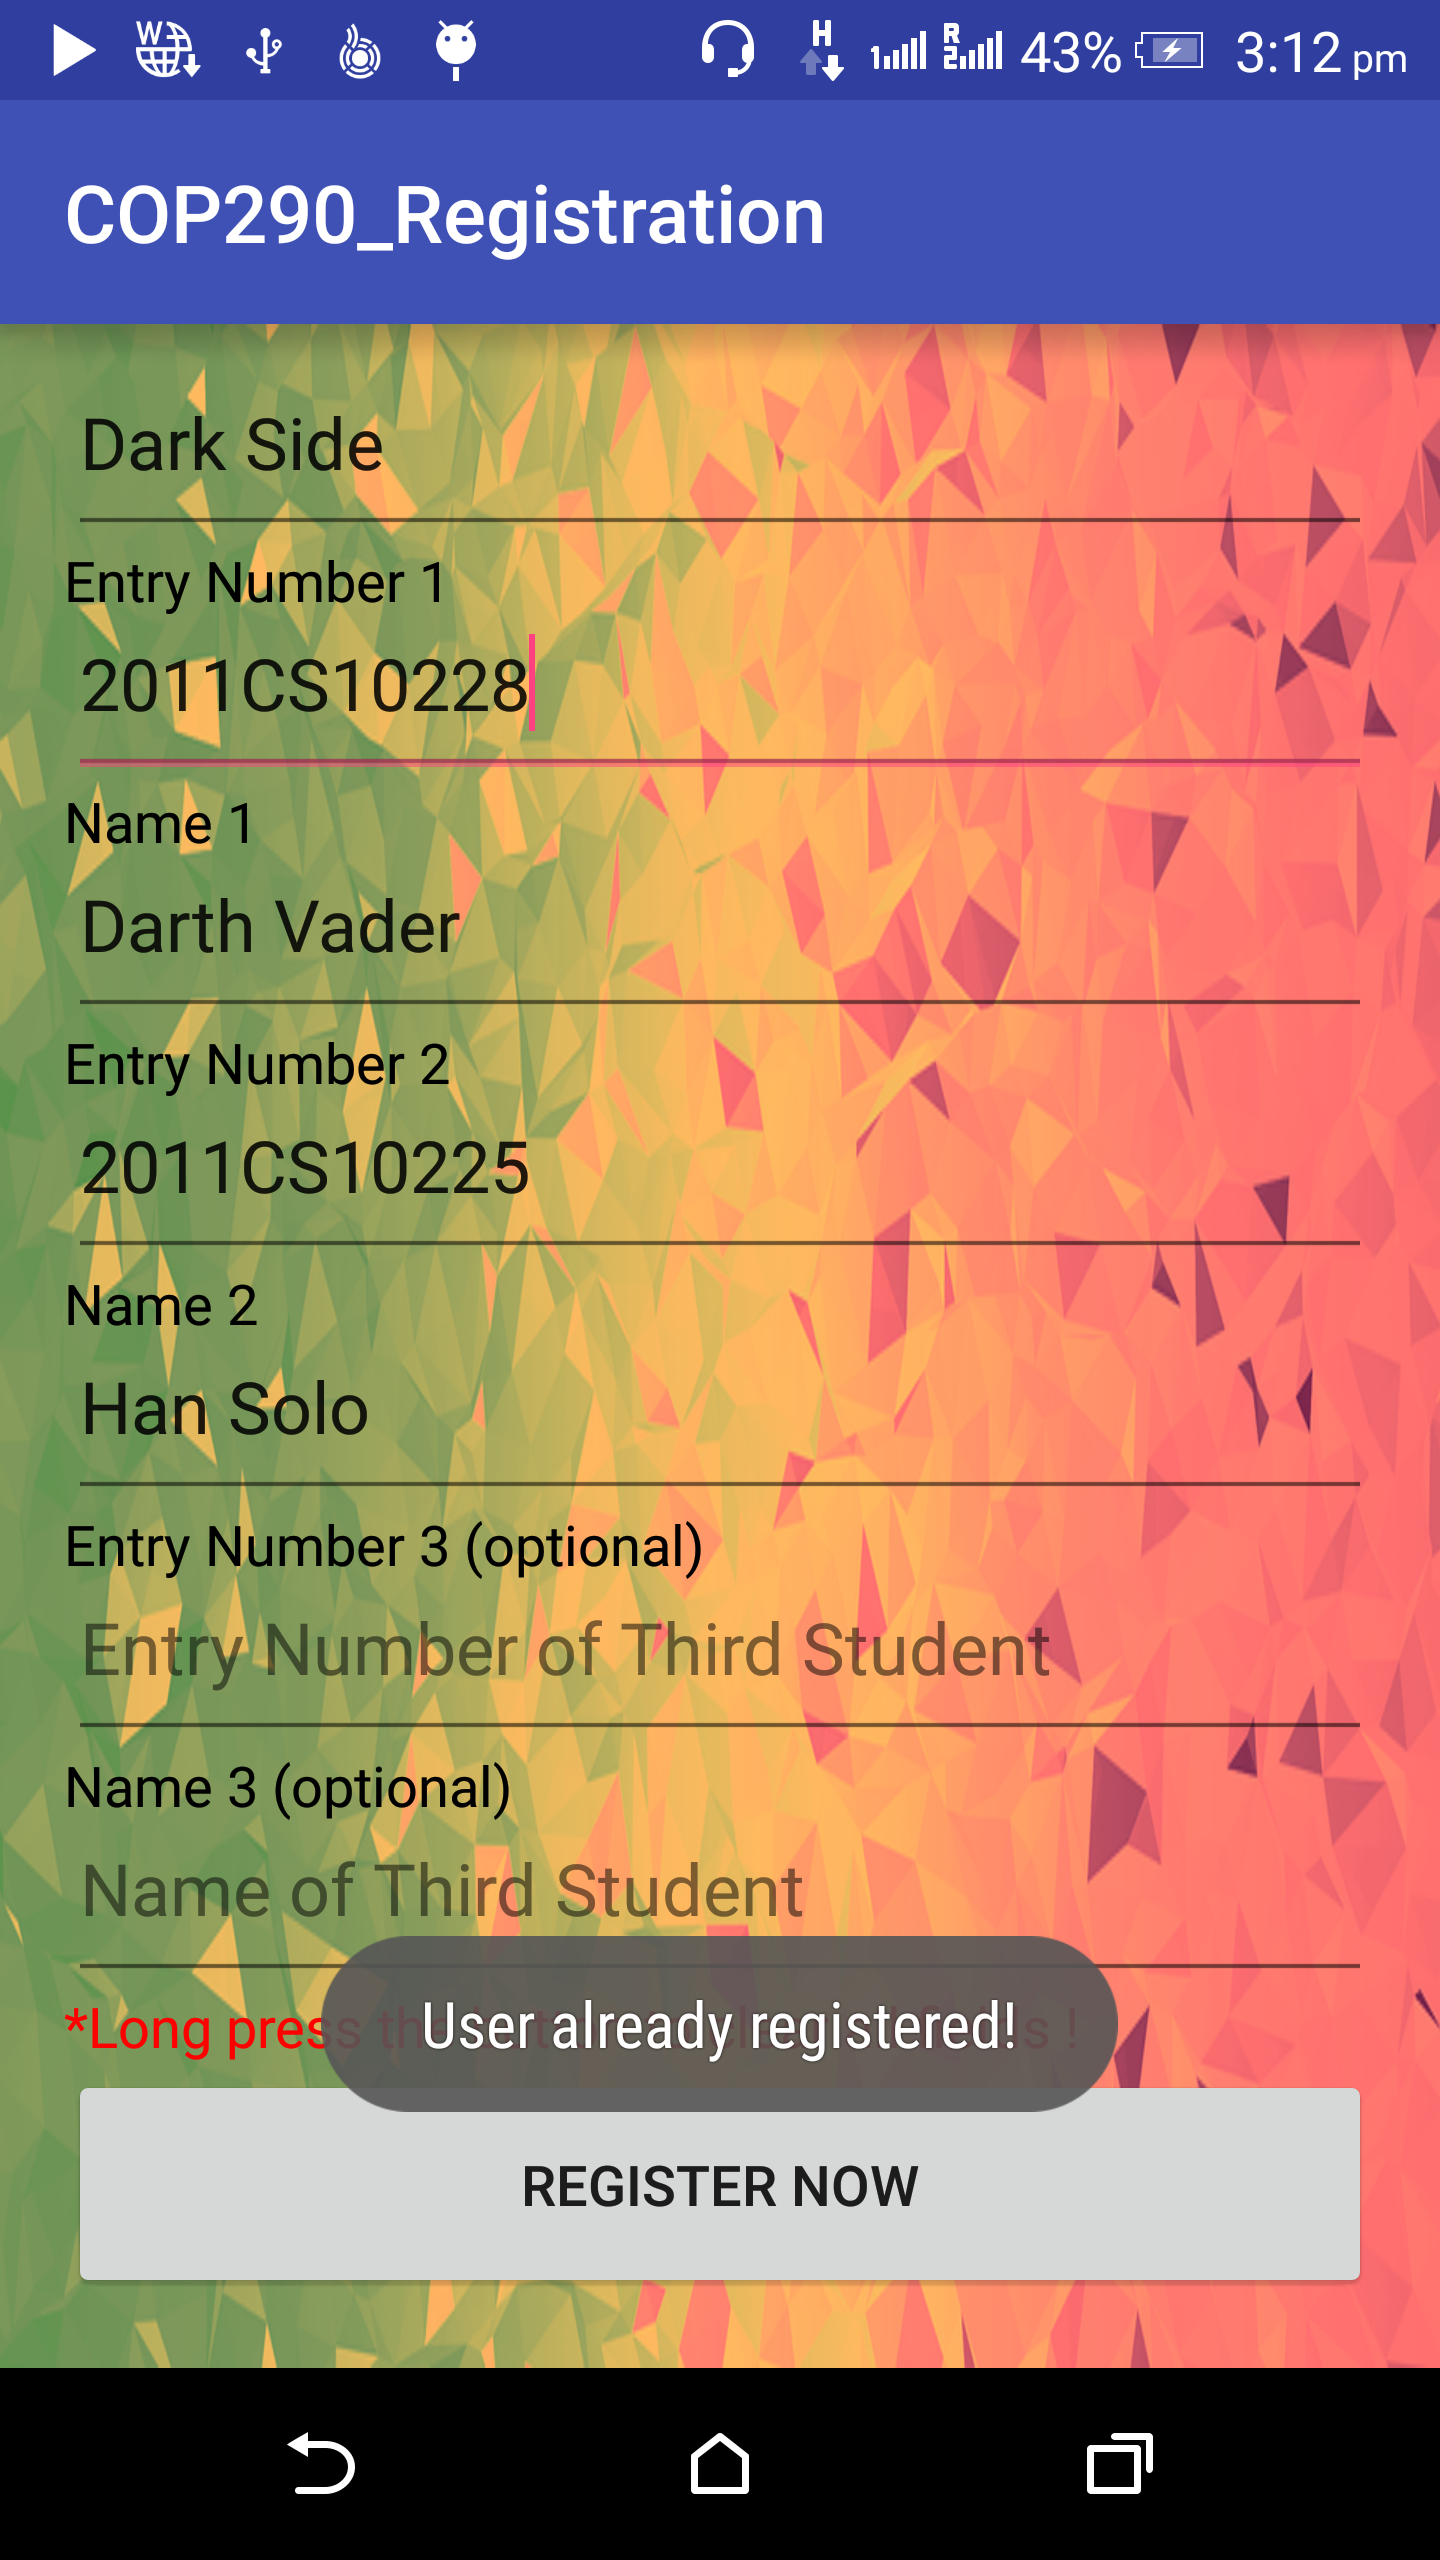
\includegraphics[width=\textwidth]{images/already.png}
    \caption{User already registered}
  \end{minipage}
\end{figure}

\FloatBarrier
\subsection{Long Press Register Button to Clear All the Fields}
Deleting text in each field can be tedious. So a new feature has been added by which all the text fields can be cleared by long pressing the register button\cite{Clearall}.
\begin{figure}[!ht]
	\centering
	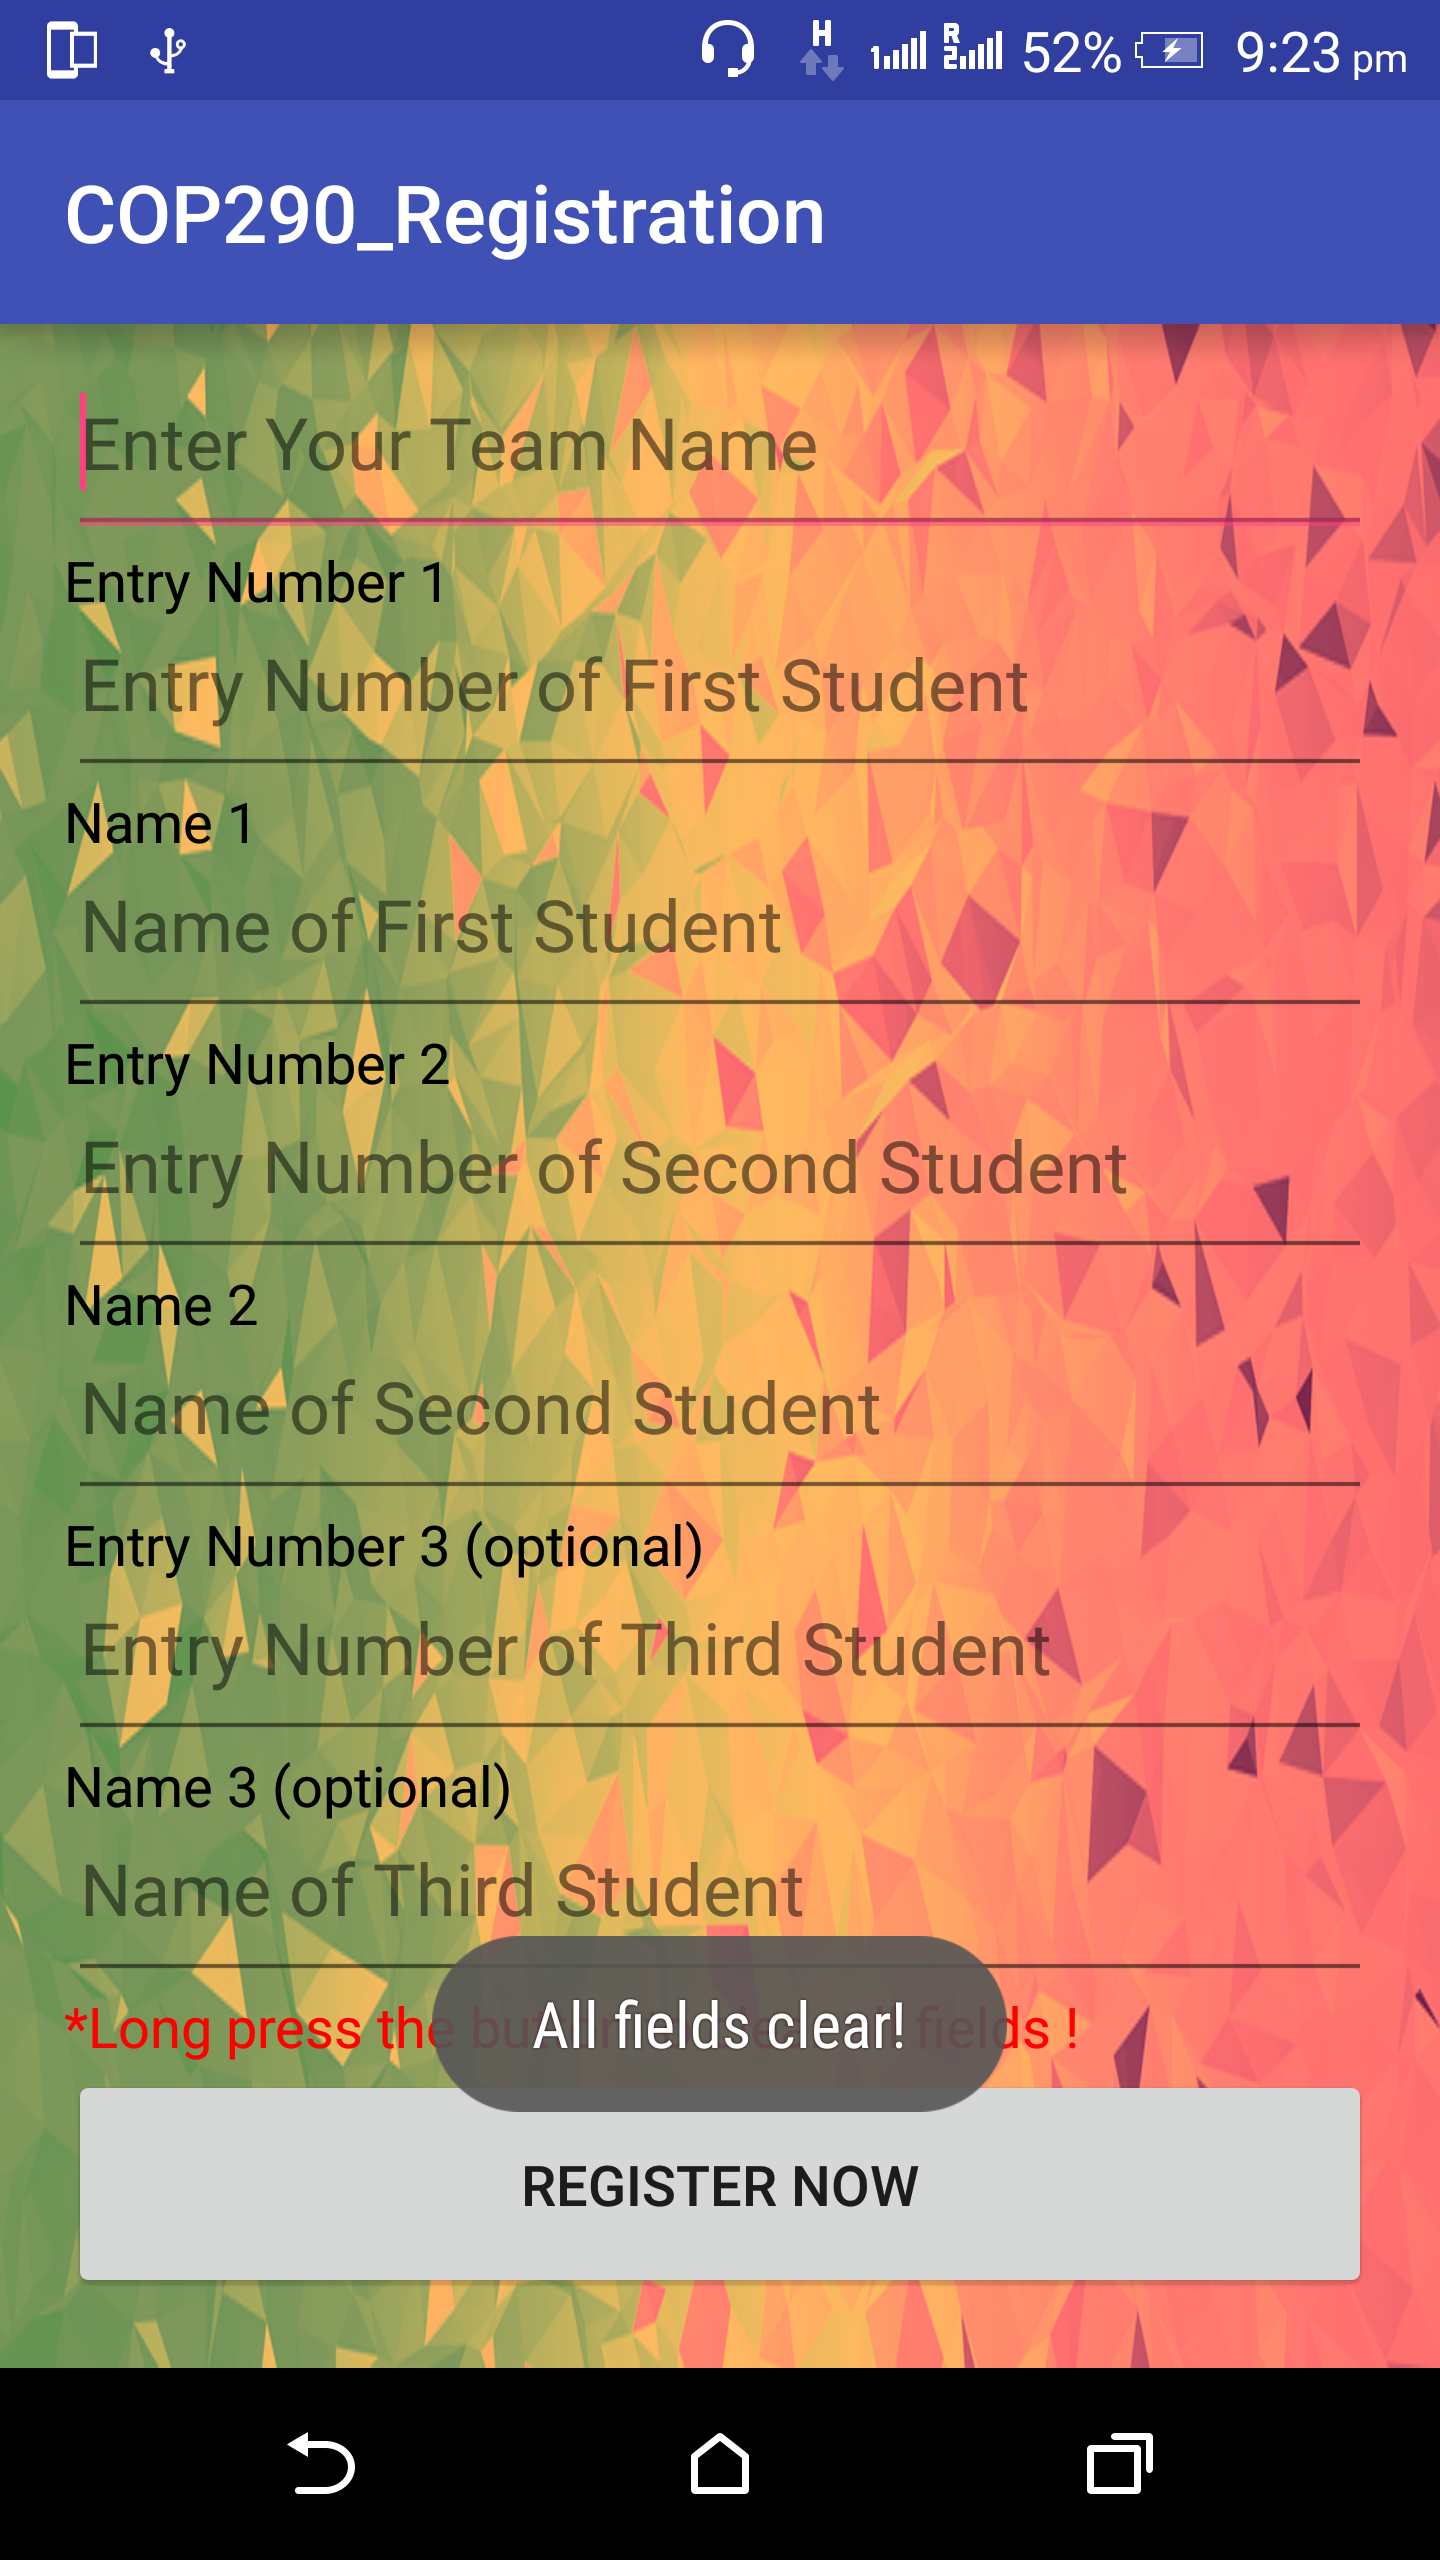
\includegraphics[width=0.5\textwidth]{images/clear.png}
	\caption{Clear Fields}
\end{figure}
\FloatBarrier  
\subsection{Press Back Button Twice to Exit the App}
When the back button is clicked to exit the application, a Toast comes up with a message \textbf{Press again to exit}\cite{Twice}.
\begin{figure}[!ht]
	\centering
	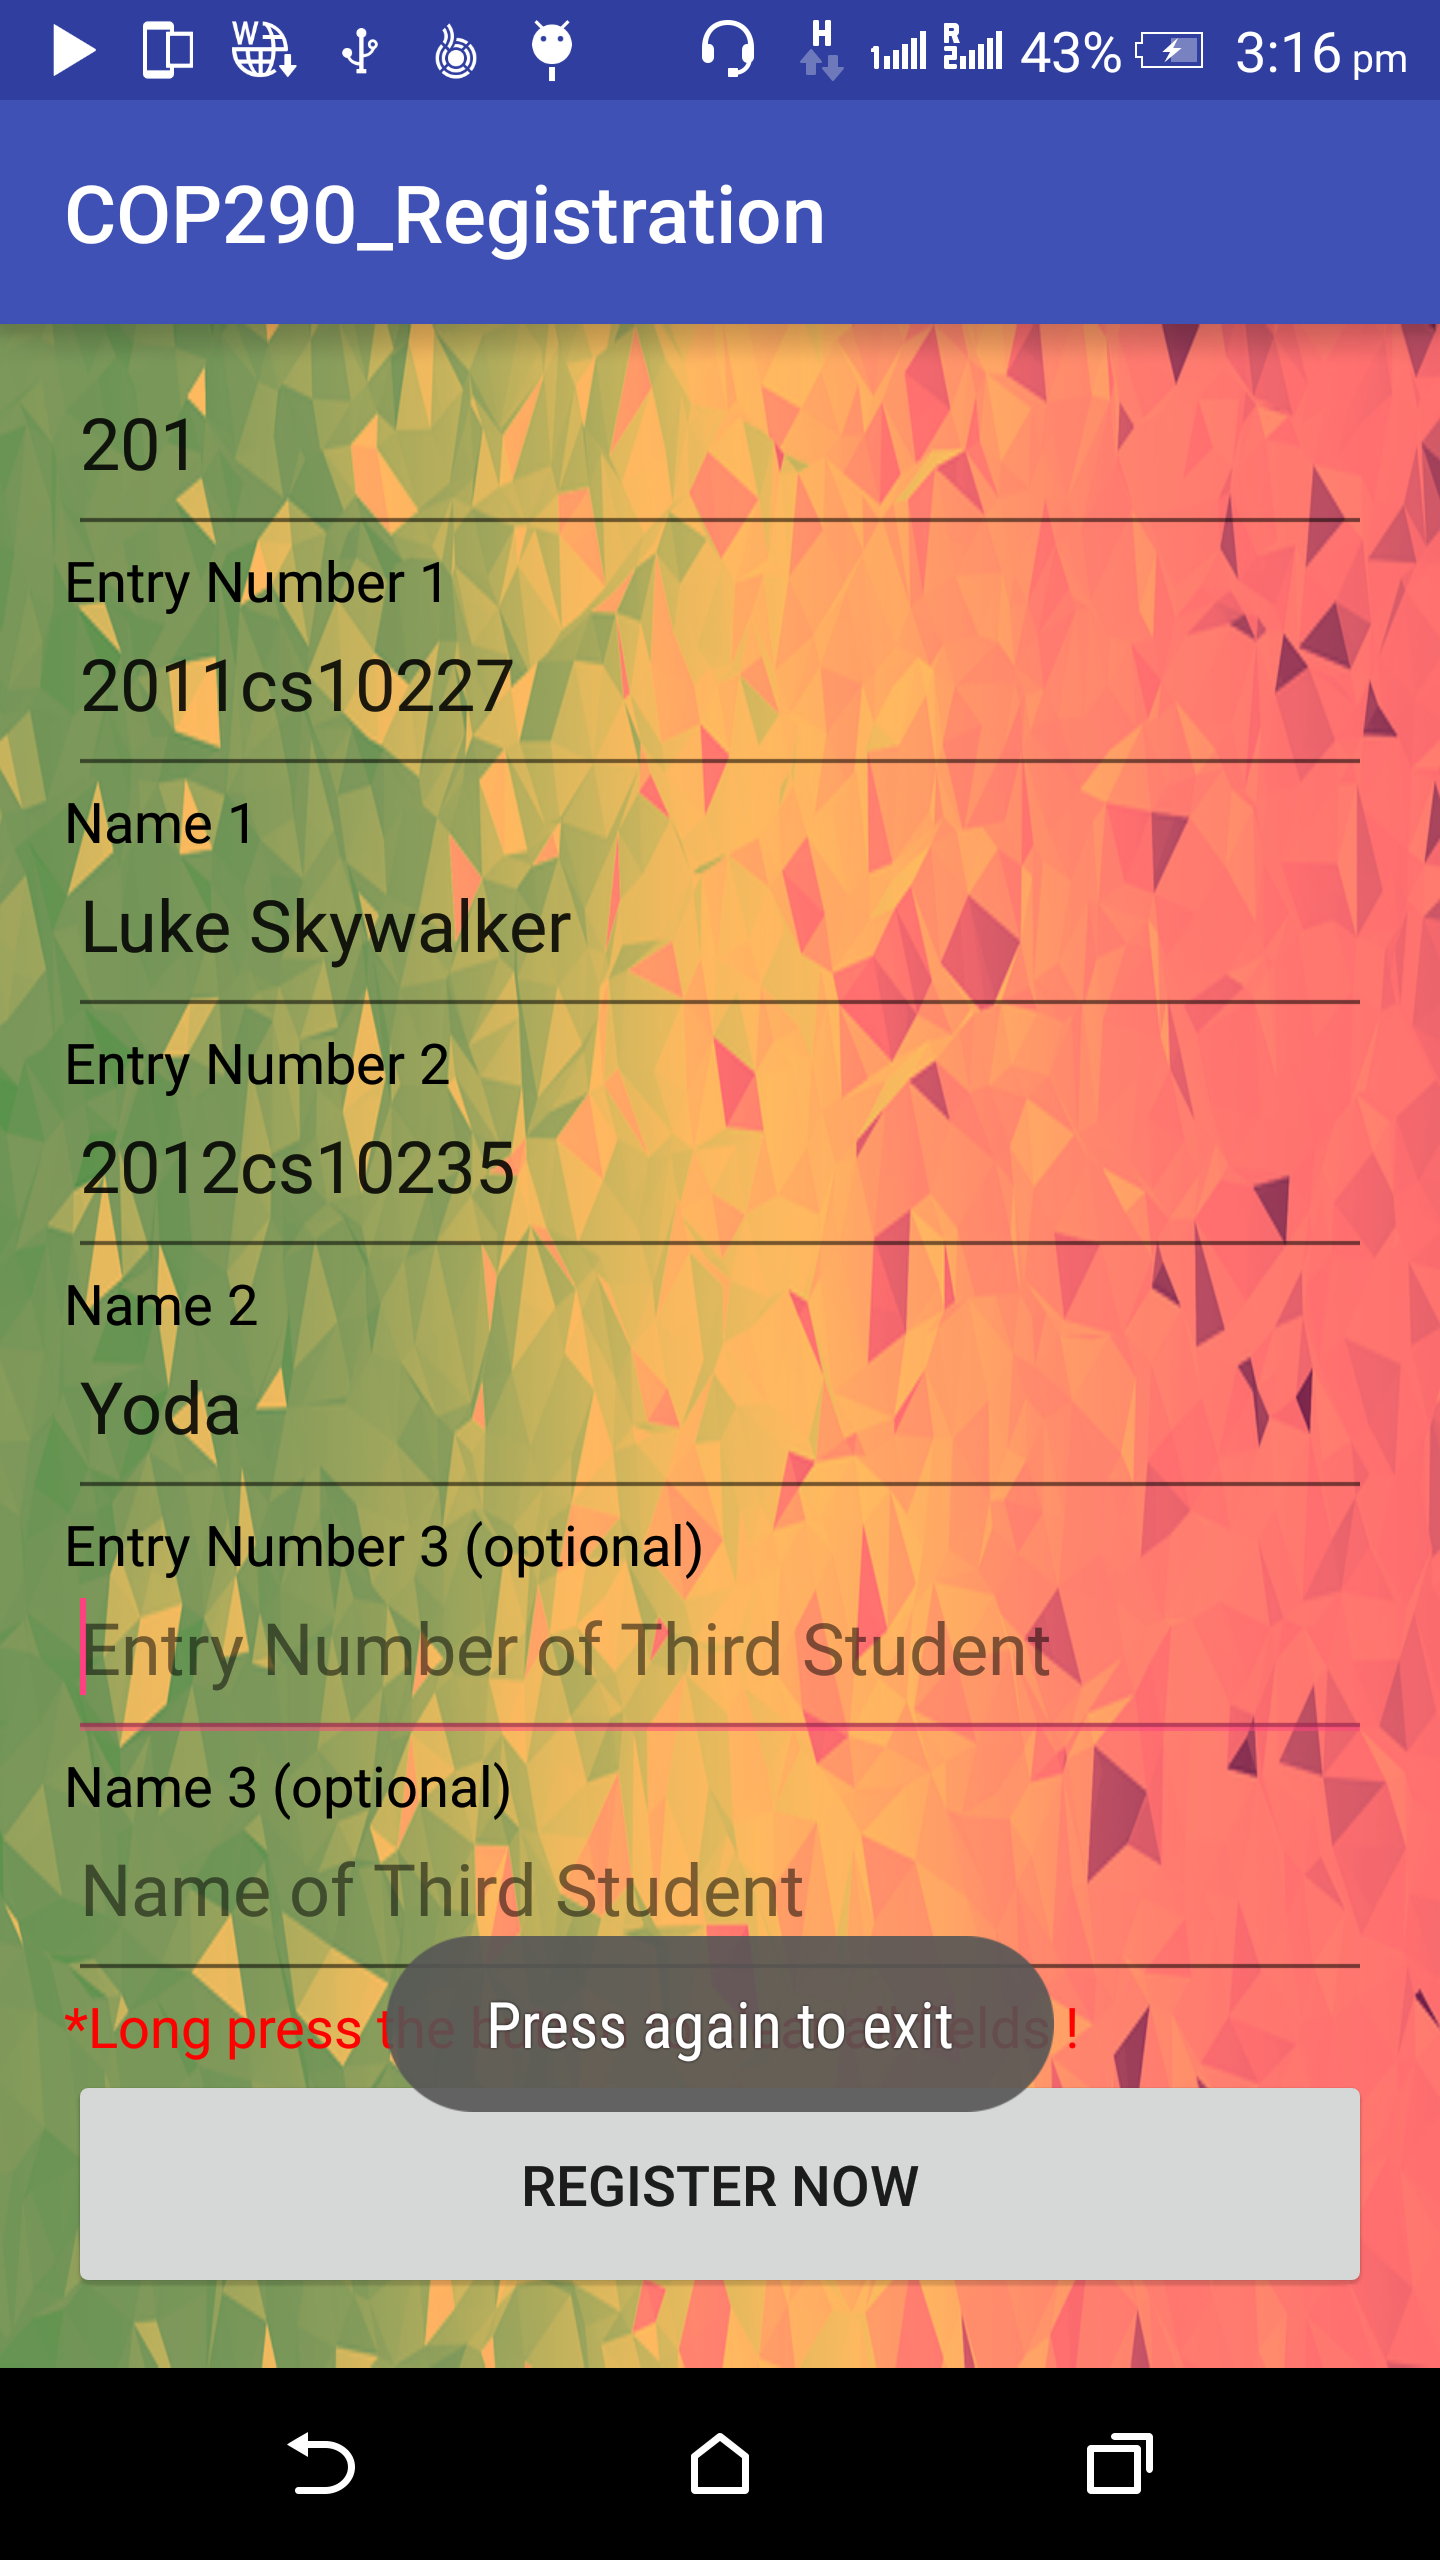
\includegraphics[width=0.5\textwidth]{images/back.png}
	\caption{Back Button Twice}
\end{figure}
\FloatBarrier
\subsection{Progress Bar}
A progress bar appears on clicking register button when all the text inputs are valid and keeps spinning till response is received from server after which it disappears.

\section{Implementation Details}
There are two classes/modules : \textbf{Main Activity} \& \textbf{Validate} . \\ \\
Main Activity consists of methods to describe what actions are to be performed on Click, longClick etc. It also contains methods for the network communications where input data is put into a hash map as (key,value) pairs and sent to the server as a string request.       
\subsection{Validation of Text Field Inputs}
\vspace{0.5cm}
\textbf{Validate} Class contains two methods - \textbf{ValidateName} \& \textbf{ValidateEntry} for validating name \& entry Number fields respectively in order to make sure that information entry is not ambiguous.
\subsubsection{ValidateName}  To make sure that the user is entering a valid entry number,
\textbf{only alphabet and spaces are allowed}. To check whether the entered text is a valid name it is matched with the following regular expression \begin{verbatim}[a-zA-Z]+( +[a-zA-Z]+)* \end{verbatim}\cite{regex}
\subsubsection{ValidateEntry}  This method is to make sure that the user is entering a valid entry number.
\begin{itemize}
\item Since COP290 is an undergraduate course, we have assumed that \textbf{PG entry numbers are invalid}. This restricts the length of entry numbers to \textbf{11 characters}.
\item Also we have restricted the domain of students registering this course to be between \textbf{2005 \& 2014} years of entry (*2005 in the worst case).
\item 2015 entry students are also ineligible to register for COP290.
\item We took into consideration the curriculum changes that took place in the years 2013 \& 2014. Following is the domain of valid branches in an entry number
\begin{itemize}
\item \textbf{UG Programs that are part of 2012 or prior Curriculum}\\
BB5, CH1, CH7, CS1, CS5, CE1, EE1, EE2, EE5, ME1, ME2, MT5, PH1, TT1;
\item \textbf{UG Programs that are part of 2013 Curriculum}\\
BB5, CH1, CH7, CS1, CS5, CE1, EE1, EE3, ME1, ME2, MT6, PH1, TT1;
\item \textbf{UG Programs that are part of 2014 Curriculum}\\
BB1, BB5, CH1, CH7, CS1, CS5, CE1, EE1, EE3, ME1, ME2, MT1, MT6, PH1, TT1;
\end{itemize}

\item Summing up all the above points , our definition of a valid entry number is the one which obeys the following rules : 
\begin{itemize}
\item Length of the entry number is 11
\item First 4 characters \textbf{(YEAR)} has to be a Valid Year (i.e 2005-2014)
\item Next 3 characters \textbf{(BRANCH)} has to be a Valid UG Programme (i.e  \em{\textbf{contains}(BRANCH,YEAR)== \textbf{true}})
\item Next 4 characters has to be a Valid Number (All digits)
\end{itemize}
\end{itemize}


\subsection{Methods for network communication}
In this assignment, we used Volley, an HTTP library that makes networking for Android applications easier
\cite{Volley}. 
\newline
\section{VCS}
The code for the project is being maintained in this repository:\\
\textbf{{\em     https://saideepbsd@bitbucket.org/saideepbsd/cop290\_a1.git}}

\bibliographystyle{abbrv}
\bibliography{references}

\end{document}
